\documentclass[tikz,convert={density=150,size=600,outext=.png}]{standalone}
\usetikzlibrary{shapes, calc, arrows, fit, positioning, decorations, patterns, decorations.pathreplacing, chains, snakes}

\begin{document}
  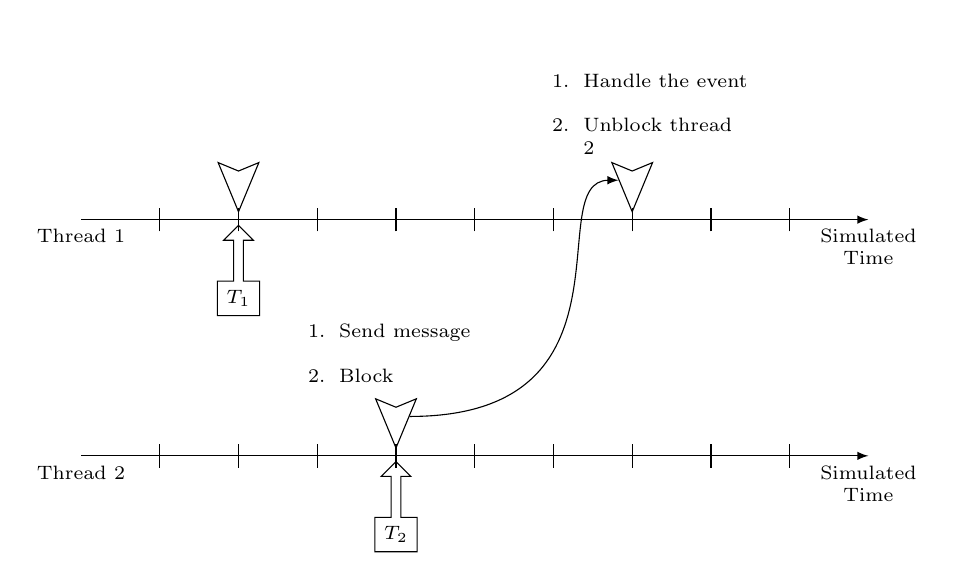
\begin{tikzpicture}[>=latex, font=\scriptsize]
    \draw[->] (0,0) -- (10,0)
      node[pos=1, below, align=center] (sim-time1) {Simulated\\Time}
      node[pos=0., below] {Thread 1};
    \foreach \x in { 1, 2, 3, 4, 5, 6, 7, 8, 9} {
      \draw (\x,-0.15) -- (\x,0.15) node (tick\x) {};
    };

    \node[draw, arrow box, arrow box arrows={north:.7cm}] at (2, -1) {$T_1$};
    \node[shape=dart, draw, shape border rotate=270 ] at (2, 0.5)  {};

    \node[shape=dart, draw, shape border rotate=270 ] at (7, 0.5) (ev-unlock) {};
    \node[above=0cm of ev-unlock, text width=3.cm, inner sep=0.2cm] {
      \begin{enumerate}
        \item Handle the event
        \item Unblock thread 2
      \end{enumerate}
    };

    \draw[->] (0,-3) -- (10,-3)
      node[pos=1, below, align=center] (sim-time2) {Simulated\\Time}
      node[pos=0., below] {Thread 2};
    \foreach \x in { 1, 2, 3, 4, 5, 6, 7, 8, 9} {
      \draw (\x,-3.15) -- (\x,-2.85) node (tick\x) {};
    };

    \node[draw, arrow box, arrow box arrows={north:.7cm}] at (4, -4) {$T_2$};

    \node[shape=dart, draw, shape border rotate=270 ] at (4, -2.5) (ev-lock) {};
    \node[text width=3.2cm, inner sep=0.2cm, above of=ev-lock] {
      \begin{enumerate}
        \item Send message
        \item Block
      \end{enumerate}
    };

    \draw[->] (ev-lock.east) .. controls +(3,0) and +(-1,0) .. (ev-unlock.west);
  \end{tikzpicture}
\end{document}
